\begin{figure}[H]
	\centering
	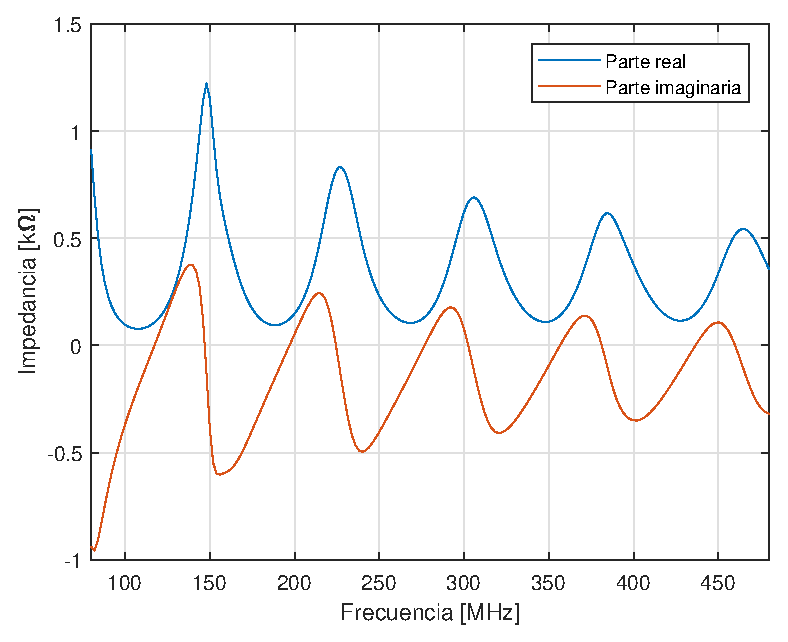
\includegraphics{imagenes/z_espacio_libre.eps}
	\caption{Resistencia de radiación.}
	\label{fig.z_radiacion}
\end{figure}

La impedancia de radiación en función de la frecuencia, se observa en la figura \ref{fig.z_radiacion}. A partir de ella se pueden deducir los valores de impedancia de entrada para las frecuencias extremas \eqref{ec.z_80} y \eqref{ec.z_480}.

\begin{equation}
	\centering
	Z(\SI{80}{\mega\hertz}) = (914 - j \cdot 930) \Omega
	\label{ec.z_80}
\end{equation}

\begin{equation}
	\centering
	Z(\SI{480}{\mega\hertz}) = (357 -j \cdot 328) \Omega
	\label{ec.z_480}
\end{equation}	

Conocer la parte imaginaria de la impedancia de la estructura resulta de utilidad si se quiere adaptar la antena a una línea de transmisión de parámetros conocidos. Si la carga que vé la antena tiene como valor su misma impedancia pero conjugada, se logra la máxima transferencia de potencia posible.